\documentclass[12pt,a4paper]{article}
\usepackage[brazil]{babel}
\usepackage[utf8]{inputenc}
\usepackage[T1]{fontenc}
\usepackage{lmodern}
\usepackage{microtype}
\usepackage{geometry}
\usepackage{graphicx}
\usepackage{tabularx}
\usepackage{booktabs}
\usepackage{longtable}
\usepackage{array}
\usepackage{enumitem}
\usepackage{setspace}
\usepackage{caption}
\usepackage{xcolor}
\usepackage{hyperref}
\usepackage{float}
\usepackage{fancyhdr}
\usepackage{amsmath}
\usepackage{url}
\usepackage{xurl}

\geometry{top=2.7cm,bottom=2.4cm,left=3cm,right=2cm}
\onehalfspacing
\setlength{\parindent}{1.25cm}
\setlength{\parskip}{0.2em}
\setlength{\headheight}{14pt}
\setlength{\emergencystretch}{2em}
\setlist[itemize]{leftmargin=1.4cm,itemsep=0.25em,topsep=0.3em}
\setlist[enumerate]{leftmargin=1.4cm,itemsep=0.25em,topsep=0.3em}
\hypersetup{colorlinks=true,linkcolor=blue!55!black,urlcolor=blue!55!black,citecolor=blue!55!black,pdftitle={Atividade XIII — PetCuida},pdfauthor={Grupo 4 — Engenharia de Computação — PUC Minas}}
\captionsetup{font=small,labelfont=bf}
\pagestyle{fancy}
\fancyhf{}
\lhead{\small PetCuida}
\rhead{\small Atividade XIII}
\cfoot{\thepage}
\renewcommand{\headrulewidth}{0.4pt}
\newcolumntype{Y}{>{\raggedright\arraybackslash}X}
\newcolumntype{P}[1]{>{\raggedright\arraybackslash}p{#1}}

\begin{document}
\selectlanguage{brazil}

\begin{titlepage}
\thispagestyle{empty}
\begin{center}

\includegraphics[width=0.19\textwidth]{assets/brasao.png}\\[0.4cm]
{\large\textbf{PONTIFÍCIA UNIVERSIDADE CATÓLICA DE MINAS GERAIS}}\\[0.15cm]
{\large Curso de Engenharia de Computação}\\
{\large Tópicos III -- Empreendedorismo e Inovação}

\vfill
{\LARGE\textbf{Atividade XIII}}\\[0.35cm]
{\Large Estratégias de crescimento, viabilidade e coerência}\\[0.25cm]
{\large Startup: PetCuida}\\[0.25cm]
{\normalsize Versão revisada, com base de evidências ampliada}

\vfill
\textbf{Integrantes}\\[0.15cm]
Gabriel da Silva Cassino\\
Giovanna Naves Ribeiro\\
Júlia Rodrigues Vasconcellos Melo\\
Kathleen Rodrigues Leite Barbosa

\vfill
\textbf{Professor-orientador:} João Carlos Oliveira Caetano\\
\textbf{Professor-tutor:} Paulo Mattos

\vfill
Belo Horizonte\\
2026
\end{center}
\end{titlepage}

\begin{titlepage}
\thispagestyle{empty}
\begin{center}
{\large Gabriel da Silva Cassino}\\
{\large Giovanna Naves Ribeiro}\\
{\large Júlia Rodrigues Vasconcellos Melo}\\
{\large Kathleen Rodrigues Leite Barbosa}

\vfill
{\Large\textbf{Atividade XIII}}\\[0.25cm]
{\large Estratégias de crescimento, viabilidade e coerência}\\[0.25cm]
{\large Startup: PetCuida}
\end{center}
\vfill
\begin{flushright}
\begin{minipage}{8.2cm}
\small\singlespacing
Trabalho acadêmico apresentado à disciplina Tópicos III -- Empreendedorismo e Inovação, do Curso de Engenharia de Computação da Pontifícia Universidade Católica de Minas Gerais, como requisito parcial de avaliação da Atividade XIII.\\[0.35cm]
\textbf{Professor-orientador:} Prof. João Carlos Oliveira Caetano\\
\textbf{Professor-tutor:} Prof. Paulo Mattos
\end{minipage}
\end{flushright}
\vfill
\begin{center}Belo Horizonte\\2026\end{center}
\end{titlepage}

\pagenumbering{roman}
\tableofcontents
\clearpage
\pagenumbering{arabic}

\section{Introdução}

Este documento apresenta o plano de crescimento e escalabilidade do PetCuida, conforme a orientação da Atividade XIII [1]. O plano segue as quatro etapas pedidas: diagnóstico do estágio atual, duas estratégias de crescimento, estratégias de escalabilidade e um plano de ação resumido com recursos e indicadores. A apresentação visual e a estrutura do pitch correspondem à Atividade XII e são entregues em arquivos separados.

Esta versão revisada reforça cada decisão do plano com fontes de quatro tipos: artigos científicos sobre acesso ao cuidado veterinário, telemedicina, usabilidade, engajamento e estratégia de startups; relatórios e dados oficiais, como o IBGE e o Conselho Federal de Medicina Veterinária; documentos do próprio grupo; e reportagens sobre a oferta pública de castração em Belo Horizonte. Quando uma fonte é um relatório de mercado ou de uma marca, ou tem limitações metodológicas conhecidas, o texto avisa. As referências estão agrupadas por tipo ao final.

O PetCuida é um projeto de aplicativo Flutter para organizar registros e lembretes do pet, apresentar uma triagem orientativa e demonstrar uma rede de serviços solidários. O repositório contém telas de protótipo e registros de testes da versão Alpha 3i [2, 3]. Por isso, o plano parte de uma regra simples: o crescimento proposto deve seguir a mesma ordem em que a equipe reduz incertezas, que é a lógica do empreendedorismo orientado por hipóteses [11].

\section{Diagnóstico do estágio atual}

\subsection{Em que fase a startup se encontra}

A recomendação é tratar o PetCuida como um protótipo em validação, na transição para um piloto de escopo pequeno. Dentro das fases pedidas (ideação, validação, tração e escala), o projeto está entre ideação e validação: existe produto demonstrável e há sinais qualitativos, mas não há usuários ativos, receita ou parceiros formalizados descritos nas fontes analisadas. A documentação de usabilidade registra limites que precisam permanecer explícitos: o mapa era esquemático, sem georreferenciamento real; o login Google estava simulado; e parte dos participantes não compreendeu de imediato os créditos ou a finalidade do QR Code [3].

\begin{table}[H]
\centering
\small
\caption{Separação entre situação observada e proposta a validar.}
\begin{tabularx}{\textwidth}{P{3.1cm}YY}
\toprule
\textbf{Dimensão} & \textbf{Base observada} & \textbf{Proposta a validar} \\
\midrule
Produto & Protótipo funcional com telas para perfil do pet, calendário, triagem e rede demonstrativa. & Piloto controlado com fluxos revistos e registro de tarefas concluídas. \\
Mercado & Cinco sessões qualitativas de usabilidade e um contexto setorial amplo. & Confirmar demanda local, frequência de uso e necessidades de clínicas e tutores. \\
Receita & Não há faturamento ou preço validado descrito nas fontes analisadas. & Testar planos para parceiros, intermediação e convênios/patrocínios, sem pressupor adesão. \\
Parcerias & Não se presumem contratos ou clínicas formalmente parceiras. & Prospectar organizações locais e medir interesse em participar de um piloto. \\
\bottomrule
\end{tabularx}
\end{table}

\subsection{Evidência inicial e limites}

O relatório do grupo registra cinco sessões com participantes de perfis variados. Os relatos foram favoráveis à facilidade de uso percebida, à triagem orientativa e à pertinência da rede solidária para barreiras como custo, transporte e acesso à castração. Também foram apontadas melhorias concretas para o sistema de créditos e o QR Code [3]. A amostra, contudo, foi pequena e não representativa; a navegação foi conduzida pelas pessoas entrevistadoras, sem tarefas autônomas, e não foi aplicada uma escala padronizada de usabilidade. Os resultados são sinais exploratórios de compreensão e aderência, não evidência de aquisição, retenção, disposição a pagar ou tração comercial.

A literatura de usabilidade ajuda a calibrar o que cinco sessões permitem concluir. O modelo de Nielsen e Landauer, que originou a regra dos cinco usuários, prevê que poucos participantes revelam boa parte dos problemas [14]. Uma simulação posterior mostrou que, em amostras de cinco, a média de problemas encontrados foi de 85\%, mas com variação de 55\% a quase 100\% entre as amostras; com dez participantes, a média subiu para 95\% e o mínimo para 82\% [13]. Uma análise mais recente concluiu que a regra dos cinco usuários subestima a amostra necessária [15]. Por isso o plano prevê dez testes com tarefas autônomas, e não apenas repetir cinco sessões.

\begin{figure}[H]
\centering
\begin{minipage}[t]{0.29\textwidth}\centering
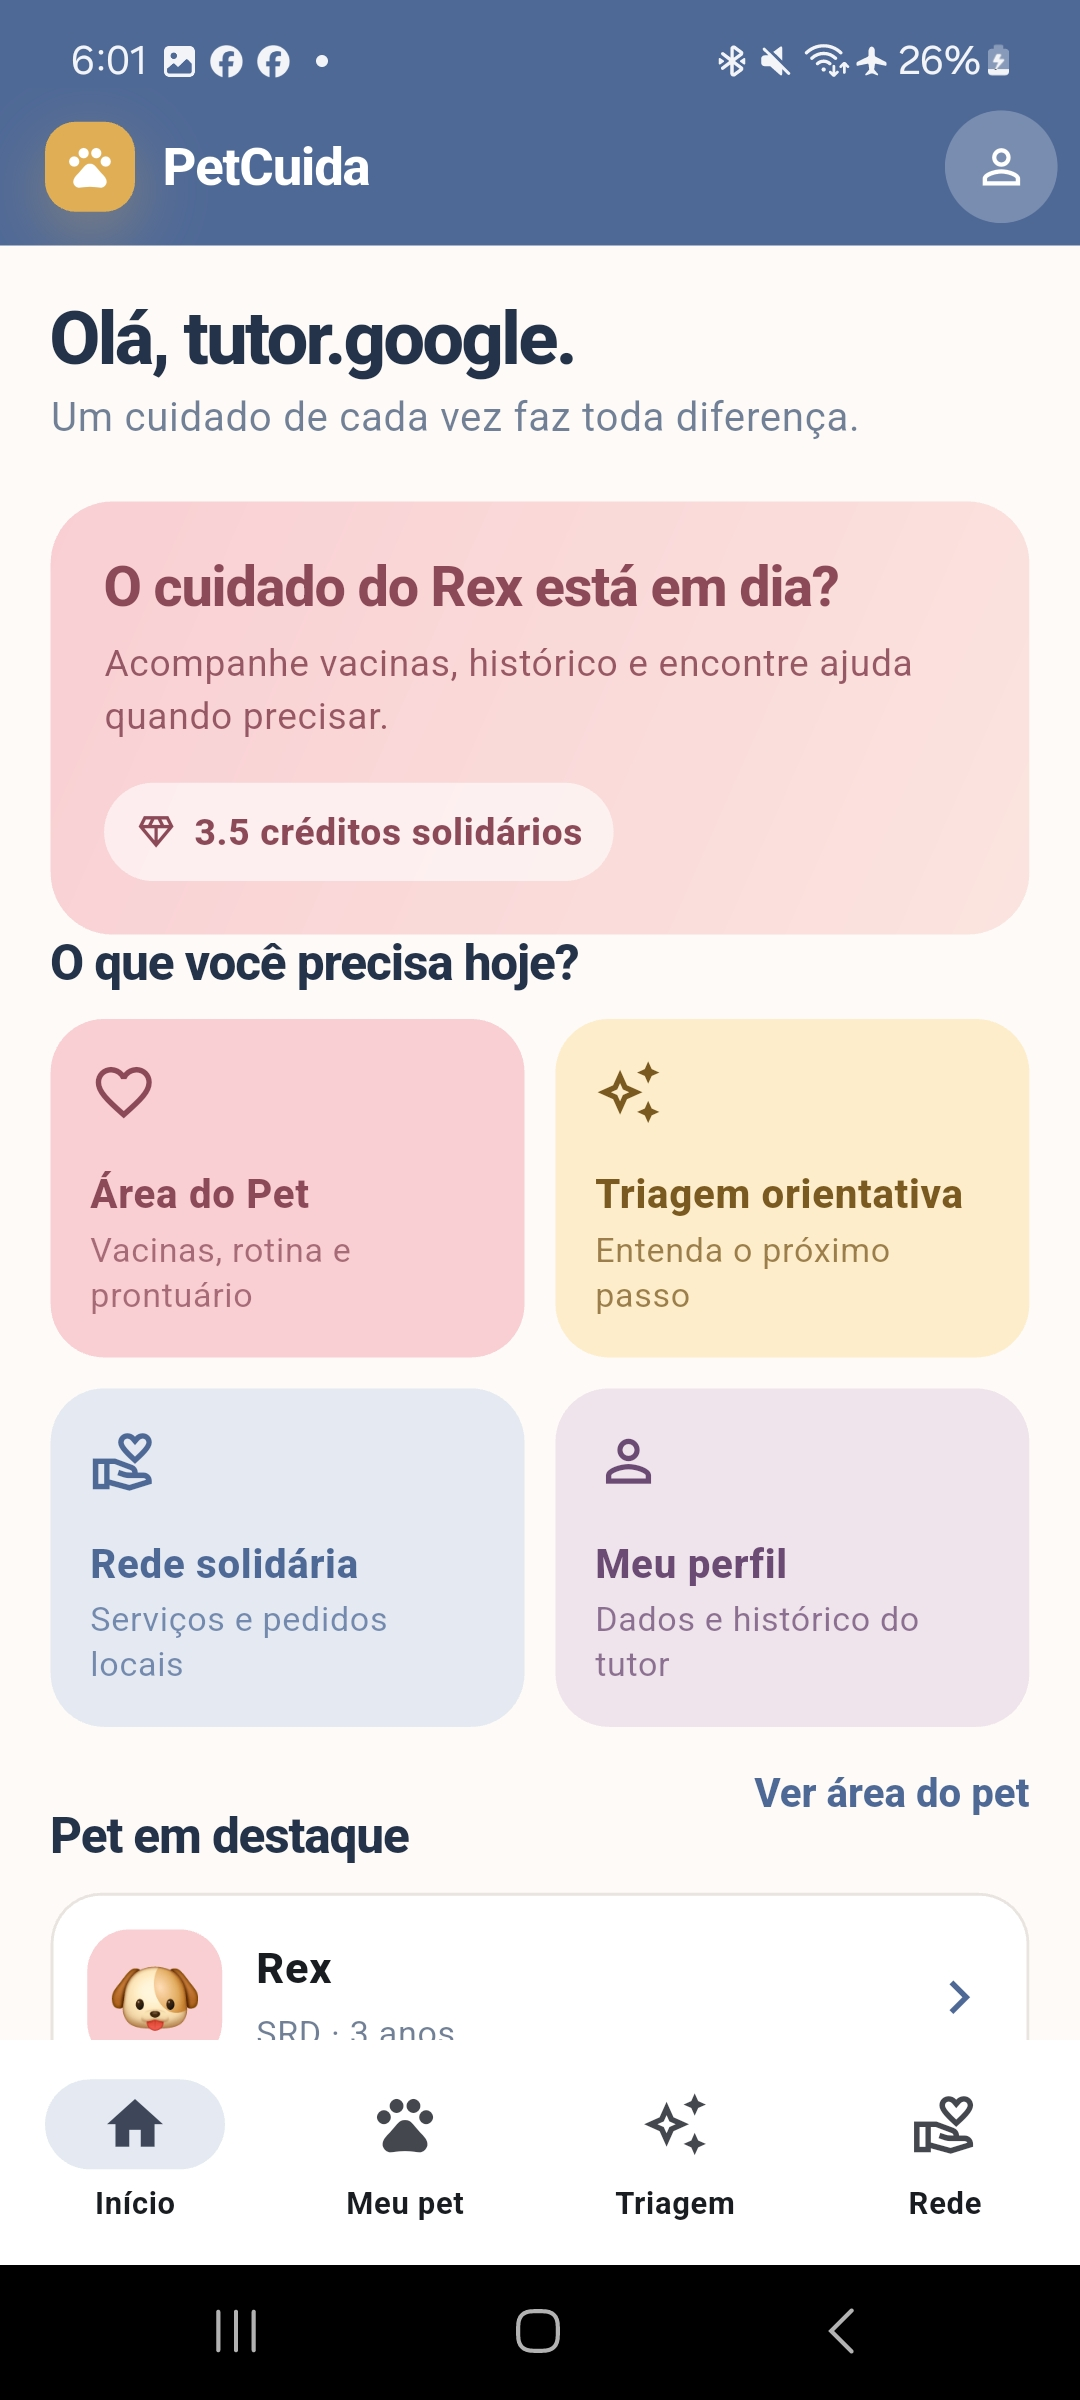
\includegraphics[height=4.7cm,keepaspectratio]{assets/tela_inicial.jpg}\\[-0.05cm]
{\small Tela inicial}
\end{minipage}\hfill
\begin{minipage}[t]{0.29\textwidth}\centering
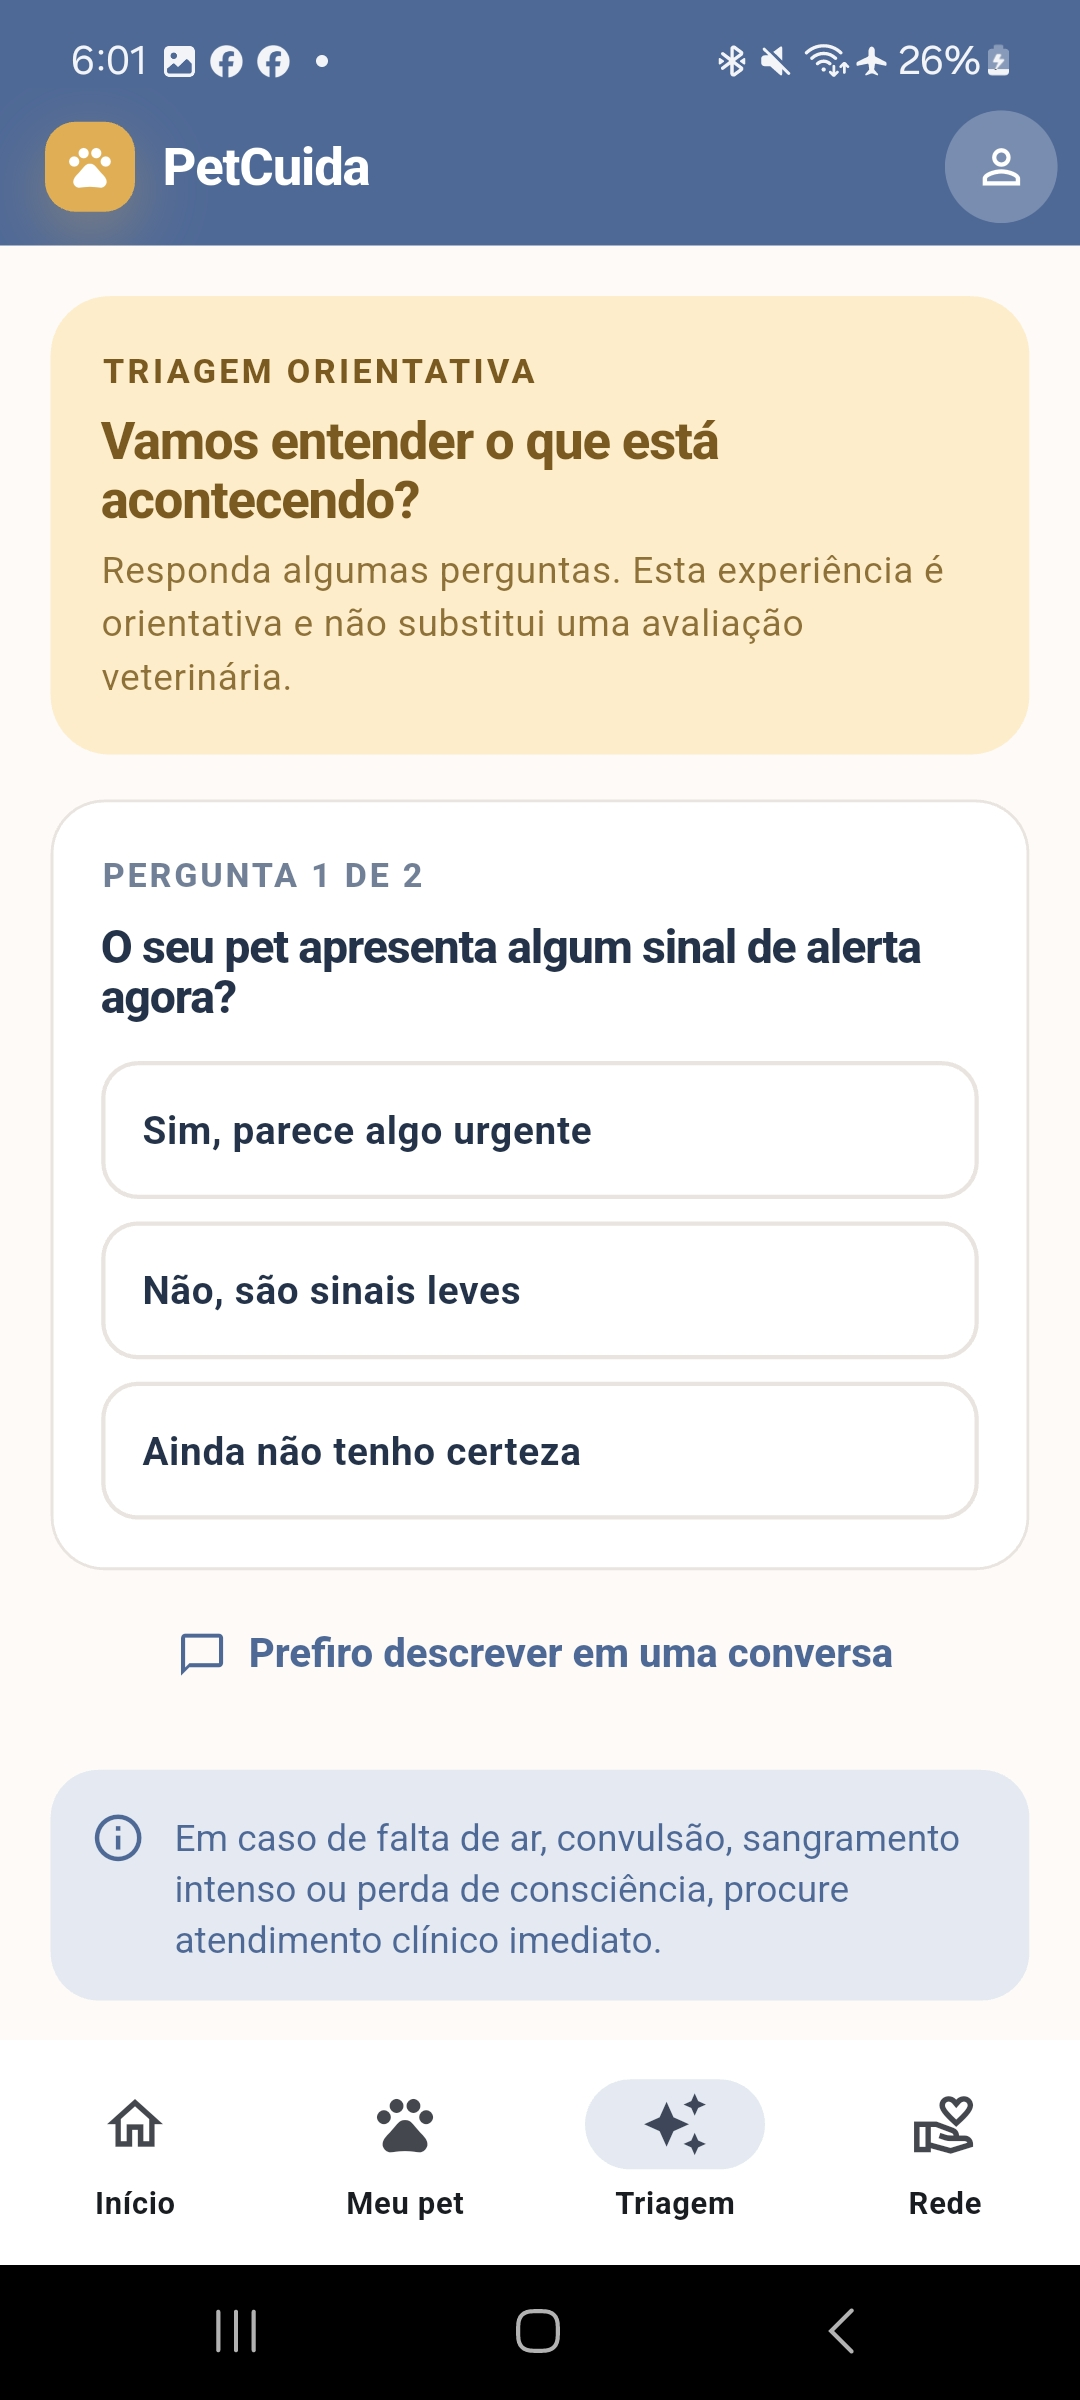
\includegraphics[height=4.7cm,keepaspectratio]{assets/tela_triagem.jpg}\\[-0.05cm]
{\small Triagem orientativa}
\end{minipage}\hfill
\begin{minipage}[t]{0.29\textwidth}\centering

\includegraphics[height=4.7cm,keepaspectratio]{assets/tela_mapa.jpg}\\[-0.05cm]
{\small Mapa demonstrativo}
\end{minipage}
\caption{Capturas do protótipo PetCuida Alpha 3i. O mapa exibido é ilustrativo, sem georreferenciamento real. Fonte: repositório do projeto [2, 3].}
\label{fig:telas}
\end{figure}

\subsection{Contexto setorial, sem confundir mercado e oportunidade}

O balanço da ABEMPET publicado em fevereiro de 2026 informa faturamento de R\$ 77,96 bilhões para o setor pet brasileiro em 2025, crescimento nominal de 3,45\% em relação a 2024. No mesmo balanço, os serviços veterinários somaram R\$ 8,18 bilhões, ou 10,5\% do total setorial [20]. Esses números indicam um setor amplo, mas não medem o mercado alcançável pelo PetCuida: incluem categorias de produtos e serviços que não correspondem necessariamente ao público, à região ou às receitas potenciais da startup. O dimensionamento local deve partir de tutores com necessidade atendível, capacidade de oferta dos parceiros e frequência de uso observada.

Do lado da demanda, a Pesquisa Nacional de Saúde 2019, do IBGE, registrou ao menos um cão em 46\% dos domicílios brasileiros e ao menos um gato em 19,3\% [19]. Uma análise da mesma pesquisa com 88.531 adultos estimou que 57,99\% possuíam cães ou gatos [18]. Esses dados mostram que ter um animal é comum, mas não dizem quantos tutores enfrentam barreiras de acesso, que é a população que o PetCuida pretende atender.

\subsection{O que a literatura diz sobre o problema}

A principal barreira ao cuidado veterinário, nos estudos disponíveis, é o custo. O relatório da Access to Veterinary Care Coalition, da Universidade do Tennessee, estimou que cerca de 28\% dos domicílios norte-americanos enfrentaram alguma barreira ao cuidado veterinário em dois anos, e que a barreira financeira predominou em todos os tipos de cuidado: 80,0\% no preventivo, 73,8\% no de doença e 55,7\% no de emergência. O mesmo relatório cita barreiras menos frequentes, como não saber onde obter atendimento e falta de transporte [21]. Uma pesquisa de 2025 da PetSmart Charities com o Instituto Gallup, com 2.498 tutores de cães e gatos, encontrou que 52\% haviam adiado ou recusado cuidado necessário [22].

Estudos revisados por pares chegam a conclusões parecidas. Em um levantamento com 177 tutores de baixa renda em Worcester (EUA), o custo foi a barreira mais bem avaliada por todos os grupos, e os clientes de uma clínica comunitária de baixo custo apresentaram melhores indicadores de cuidado preventivo do que os que não a usavam [7]. Esse desenho é de levantamento, portanto mostra associação e não prova que a clínica causou a diferença. Uma revisão sistemática concluiu que existe uma lacuna de cuidado em comunidades de baixa renda e que clínicas de baixo preço e comunitárias são uma estratégia usada para ampliar o cuidado preventivo e a castração [8]. Um estudo qualitativo com 12 tutores de baixa renda no Canadá descreveu barreiras de acesso a clínicas privadas e apontou sugestões como planos de pagamento e preços compassivos [6]. Por ser uma amostra pequena e intencional, esse resultado ilustra experiências e não pode ser generalizado.

Essas evidências vêm sobretudo de países de renda alta. Elas sustentam a hipótese central do PetCuida, mas não substituem a validação com tutores de Belo Horizonte. O próprio relatório de usabilidade do grupo registra relatos de custo e deslocamento [3], o que é coerente com a literatura, sem equivaler a medi-los na população local.

\subsection{Contexto local: a oferta pública de castração em Belo Horizonte}

A Prefeitura de Belo Horizonte oferece castração gratuita de cães e gatos com dono em centros de esterilização, com agendamento pelo Portal de Serviços [26]. Em janeiro de 2023, as 3 mil vagas abertas para fevereiro se esgotaram em cerca de três horas; a Secretaria de Saúde informou que a agenda abre uma vez por mês e que não há fila de espera, e tutores relataram dificuldade de acesso ao site e ao telefone [27]. Uma audiência na Câmara Municipal em 2021 já registrava que a rede, com um centro de zoonoses, cinco centros de esterilização e uma unidade móvel, não conseguia atender a demanda [29]. Em julho de 2026, a Prefeitura e o Instituto Arbo lançaram o Projeto Bora Bicho, com 4 mil cirurgias gratuitas em dez meses em um castramóvel, priorizando territórios de maior vulnerabilidade social e exigindo agendamento prévio [28].

Para o PetCuida, isso tem duas consequências. Primeiro, há demanda pública visível por castração a preço zero, o que reforça a relevância do problema em Belo Horizonte. Segundo, o serviço público é um possível complemento, não um concorrente: parte do problema é informação e coordenação, como saber quando a agenda abre e onde há vaga. Lembretes de abertura de agenda e orientação sobre o fluxo são uma hipótese de valor a testar com tutores, sem prometer vagas que o aplicativo não controla. Qualquer contato com a Prefeitura ou com o Instituto Arbo deve ser tratado como prospecção, não como parceria existente.

\subsection{Principais desafios para o crescimento}

\begin{itemize}
\item \textbf{Clareza da experiência:} créditos e QR Code não foram compreendidos por parte dos participantes [3].
\item \textbf{Uso autônomo ainda não testado:} a navegação foi conduzida pelas pessoas entrevistadoras.
\item \textbf{Oferta local:} sem clínicas e organizações dispostas a receber encaminhamentos, a rede solidária não entrega valor ao tutor.
\item \textbf{Economia do serviço:} não há estimativa confiável de custos de suporte, pagamento e operação.
\item \textbf{Limites clínicos, regulatórios e de dados:} a triagem é orientativa, a telemedicina veterinária é regulada pelo CFMV e o uso de dados de tutores exige cuidados de segurança e consentimento [23, 24].
\item \textbf{Dois lados do mercado:} o aplicativo só entrega valor se tutores e prestadores de serviço aparecerem juntos, o clássico problema de partida de redes de dois lados [12].
\end{itemize}

\subsection{Síntese: como as evidências orientam o plano}

\begin{table}[H]
\centering
\small
\caption{Evidências externas e seus efeitos sobre o plano.}
\begin{tabularx}{\textwidth}{P{3.4cm}YY}
\toprule
\textbf{Fonte} & \textbf{O que mostra} & \textbf{Efeito no plano} \\
\midrule
AVCC e Gallup [21, 22] & Custo é a barreira dominante, também em renda média. & Piloto sem cobrança ao tutor; foco em tutores com barreira de custo. \\
Mueller et al. [7]; LaVallee et al. [8] & Cuidado comunitário e preventivo associa-se a melhores indicadores. & Conteúdo preventivo como porta de entrada da Estratégia 2. \\
Itatiaia e PBH [26, 27, 28] & Vagas públicas de castração esgotam e dependem de agendamento. & Testar valor de orientação e lembretes sobre canais públicos. \\
Faulkner [13]; Cazañas et al. [15] & Cinco usuários podem não bastar. & Dez testes autônomos antes do piloto. \\
Baumel et al. [16] & Retenção em 30 dias costuma ser baixa em apps abertos. & Meta D30 ambiciosa, a recalibrar. \\
CFMV [23] & Teleorientação veda diagnóstico e conduta terapêutica. & Triagem educativa, revisão veterinária e consulta ao CRMV-MG. \\
Eisenmann et al. [11, 12] & Hipóteses testadas por ciclos; redes de dois lados exigem escolher o lado a subsidiar. & Ciclos de oito semanas com decisão ao fim; oferta local primeiro. \\
\bottomrule
\end{tabularx}
\end{table}

\section{Estratégias de crescimento}

\subsection{Estratégia 1: piloto territorial com operação assistida}

A primeira estratégia é uma expansão de mercado controlada: testar o fluxo em Belo Horizonte, começando em um bairro ou rede comunitária que a equipe consiga acompanhar. Antes de abrir o piloto, a equipe deve entrevistar de 15 a 20 tutores, conversar com cinco clínicas e mapear duas organizações comunitárias. Esses números são metas de pesquisa propostas, não contatos já realizados. O grupo deve registrar necessidades, horários, critérios de preço social, restrições de transporte e condições para encaminhamento.

Na segunda etapa, a equipe deve revisar a explicação dos créditos e do QR Code e testar tarefas com participantes operando o aplicativo por conta própria. Na terceira, pode executar por até oito semanas um piloto concierge, em que cadastro de parceiros e encaminhamentos sejam acompanhados manualmente. Um grupo inicial de 40 a 50 tutores e duas ou três clínicas é uma hipótese de escala de teste, condicionada a consentimento, capacidade de acompanhamento e oferta real. Não se deve apresentar essas metas como compromissos já assumidos.

O desenho segue a lógica do empreendedorismo orientado por hipóteses: formular o que precisa ser verdade para o negócio funcionar, testar com custo baixo e decidir, ao final de cada ciclo, entre perseverar, mudar parte do modelo ou abandonar [11]. Como o PetCuida conecta tutores e prestadores, a literatura sobre redes de dois lados trata como central decidir qual lado subsidiar e por quanto tempo [12]. No piloto, o tutor não paga e a oferta é construída parceiro a parceiro, começando pelo lado mais escasso, que é a disponibilidade de serviço.

As organizações públicas e sociais que já atuam em Belo Horizonte entram na etapa de mapeamento como possíveis complementos: o Portal de Serviços da Prefeitura [26] e o Projeto Bora Bicho [28] concentram demanda por castração gratuita, e o PetCuida pode testar se orientar o tutor sobre esses canais gera valor. A conversa com esses atores deve ser tratada como prospecção.

\subsection{Estratégia 2: aquisição local baseada em confiança}

A segunda estratégia combina marketing de aquisição e parcerias locais: crescer por conteúdo útil e indicação de atores locais, em vez de comprar alcance antes de provar ativação e retorno. Conteúdo de prevenção deve ser curto, revisado e explícito sobre os limites da triagem. A escolha por prevenção tem respaldo na associação encontrada entre uso de uma clínica comunitária e melhores indicadores de cuidado preventivo [7], embora esse resultado não prove causalidade. Um QR ou link diferente por parceiro ou evento permite acompanhar a origem do cadastro. O funil deve medir alcance qualificado, cadastro, criação do perfil do pet, primeiro lembrete, uso posterior e procura efetiva por serviço.

A métrica não deve ser somente o número de downloads. A ativação pode ser definida como criação de perfil do pet e registro de pelo menos um lembrete nos primeiros sete dias. A retenção no dia 30 deve considerar uma ação relevante, como consultar o prontuário, atualizar cuidado preventivo ou iniciar um encaminhamento. Campanhas pagas só devem ser consideradas após a equipe entender a conversão e o custo por tutor ativado. Também é preciso prever canal alternativo para quem tem acesso limitado a celular ou internet, como contato presencial em parceiros ou mensagem simples, porque um estudo com clientes de baixa renda de uma clínica comunitária tratou a exclusão digital como fator a avaliar ao levar atendimento remoto a essa população [9].

\section{Estratégias de escalabilidade}

\subsection{Escala operacional e tecnológica}

A escala deve ocorrer por território, não por publicidade ampla. Primeiro, padronizar cadastro do parceiro, descrição de serviços, horários, critérios de preço social, processo de encaminhamento e canal para problemas. Depois, automatizar apenas tarefas repetitivas e compreendidas, como lembretes consentidos e atualização de disponibilidade. A localização em mapa, a agenda e a intermediação financeira dependem de integração real, testes e regras de operação; a tela atual não comprova essas capacidades.

Uma vez padronizado, o modelo pode ser replicado em novos territórios com custo adicional menor, desde que cada nova região entre apenas com oferta mínima de parceiros e economia unitária compreendida. Franquias ou licenciamento não são propostos nesta fase, pois dependem de processo estável e de revisão jurídica.

Antes de usar dados de tutores em piloto, a equipe deve definir finalidade, base e forma de consentimento aplicáveis, limitar coleta, controlar acessos, proteger cópias de segurança e estabelecer um procedimento de resposta a incidentes. O guia da ANPD para agentes de tratamento de pequeno porte oferece uma referência prática de medidas organizacionais e técnicas [24], e o tratamento de dados pessoais de tutores está sujeito à Lei Geral de Proteção de Dados [25]. As recomendações devem ser revisadas à luz do produto real e das obrigações aplicáveis antes de qualquer implantação pública.

\subsection{Limites regulatórios e clínicos da triagem}

A Resolução CFMV nº 1.465/2022 regulamenta a telemedicina veterinária e define a teleorientação como orientação geral e inicial à distância, com vedação a qualquer definição diagnóstica ou conduta terapêutica. A norma restringe as modalidades de telemedicina a médicos-veterinários com inscrição ativa no sistema CFMV/CRMVs, exige que o profissional avise previamente, na teleorientação e na teletriagem, que não se trata de consulta, e condiciona a teleconsulta a um vínculo presencial prévio com o responsável pelo animal [23]. Como a norma disciplina atos de médicos-veterinários, o grupo deve consultar o CRMV-MG e assessoria jurídica sobre como enquadrar uma triagem automatizada. Até lá, o texto da triagem deve permanecer educativo, sem diagnóstico nem conduta terapêutica, e ser revisado por médico-veterinário.

Esse cuidado combina com o que mostram as revisões da área. Um resumo de conhecimento com oito estudos encontrou evidência fraca de satisfação semelhante entre teleconsulta e consulta presencial e considerou a aplicação ainda limitada a cenários selecionados [10]. A telemedicina não deve, portanto, ser apresentada como substituta do atendimento presencial.

\subsection{Evitar a escala prematura}

Um relatório do Startup Genome, com dados de mais de 3.200 startups de tecnologia, associou o desempenho pior à escala prematura, definida como avançar em equipe, produto ou captação antes de o estágio do negócio justificar [17]. O relatório foi produzido por uma empresa de benchmarking, não passou por revisão por pares e foi criticado por seu raciocínio circular, então serve como alerta e não como prova. Ele reforça a regra do plano: ampliar território somente após cumprir os critérios de decisão do piloto.

\subsection{Viabilidade econômica e receita recorrente}

Não há base confiável no material analisado para estimar preço, receita, custo de aquisição, custo de suporte ou ponto de equilíbrio. Por isso, esta versão não projeta faturamento. A avaliação deve começar com uma planilha simples de custos fixos mensais, taxas de pagamento, hospedagem, comunicação, atendimento e tempo da equipe. O custo do tempo dos fundadores deve ser registrado, mesmo que não haja desembolso imediato, para não mascarar a economia do serviço.

O modelo descrito na Atividade X considera assinaturas, planos para parceiros, intermediação de atendimentos e convênios ou patrocínios como possibilidades [4]. Aqui, essas vias são mantidas como hipóteses independentes. No piloto, não cobrar usuários, não intermediar dinheiro sem processo definido e não contabilizar patrocínios antes de existir compromisso formal.

Como instrumento para a próxima análise, a receita mensal pode ser representada por:
\[
\text{Receita mensal} = (N_c \times P_c) + (N_a \times T_a) + S,
\]
onde $N_c$ é o número de clínicas pagantes, $P_c$ é o preço mensal do plano parceiro, $N_a$ é o número de atendimentos concluídos por intermediação, $T_a$ é a receita líquida por atendimento e $S$ é o patrocínio ou convênio mensal. As variáveis só devem ser preenchidas quando existirem propostas testadas e registros reais.

A margem de contribuição deve descontar custos variáveis de pagamentos, atendimento e operação. Para margem média positiva por parceiro, o número de parceiros pagantes necessário ao equilíbrio pode ser estimado por:
\[
N_{\text{equilíbrio}} = \frac{\text{custos fixos mensais}}{\text{margem média de contribuição por parceiro}}.
\]
Se a margem for nula ou negativa, a hipótese deve ser revista antes de ampliar a operação. O cálculo é um método a aplicar após a coleta de dados, não um resultado desta atividade.

\begin{table}[H]
\centering
\small
\caption{Hipóteses de receita e critérios mínimos de validação.}
\begin{tabularx}{\textwidth}{P{3.0cm}YY}
\toprule
\textbf{Hipótese} & \textbf{Como testar sem presumir adesão} & \textbf{Critério para avançar} \\
\midrule
Plano para parceiros & Entrevistar clínicas sobre problema, valor esperado, rotina de uso e faixa de preço. & Ao menos duas clínicas aceitam novo ciclo de teste e participam de conversa de preço. \\
Intermediação & Medir encaminhamentos, conclusão, suporte e custo operacional em processo acompanhado. & Fluxo rastreável, regras claras e custo variável conhecido; revisão jurídica antes de cobrar. \\
Patrocínio ou convênio & Apresentar proposta delimitada a empresas ou organizações locais. & Só incluir receita após manifestação formal e condições de uso definidas. \\
Assinatura para tutor & Testar interesse sem bloquear funções essenciais de cuidado preventivo. & Evidência de valor recorrente e intenção de pagamento; não lançar por suposição. \\
\bottomrule
\end{tabularx}
\end{table}

\section{Plano de ação resumido}

O quadro a seguir reúne a estratégia principal de crescimento, as ações-chave, os recursos necessários e os indicadores de sucesso, conforme pedido na orientação [1]. A estratégia principal é o piloto territorial em Belo Horizonte; a aquisição baseada em confiança entra como apoio à ativação dos tutores.

\begin{table}[H]
\centering
\small
\caption{Quadro-resumo do plano de ação.}
\begin{tabularx}{\textwidth}{P{2.7cm}YYY}
\toprule
\textbf{Estratégia} & \textbf{Ações-chave} & \textbf{Recursos necessários} & \textbf{Indicadores de sucesso} \\
\midrule
Piloto territorial (principal) & Entrevistas e mapeamento local; revisão de créditos e QR; teste autônomo; piloto concierge de oito semanas. & Horas dos quatro integrantes; roteiros e termo de consentimento; ambiente de teste do app; planilha de custos; contato com clínicas e organizações. & 10 testes com 8 conclusões sem ajuda [13]; 80\% explicam créditos e QR; 2 clínicas aceitam novo ciclo. \\
Aquisição por confiança (apoio) & Conteúdo preventivo revisado; QR ou link por parceiro; funil de cadastro até primeiro lembrete. & Material de comunicação simples; revisão de conteúdo por pessoa qualificada, a definir; painel básico de métricas. & Ativação de 60\%; retenção D30 de 30\%; custo por tutor ativado registrado. \\
Escalabilidade & Padronizar ficha de parceiro; automatizar lembretes consentidos; definir regras de créditos. & Documentação de processos; ajustes de back-end; revisão de segurança e de regras de créditos e repasses. & Tempo de cadastro de parceiro; custo de suporte por tutor; margem de contribuição por parceiro. \\
\bottomrule
\end{tabularx}
\end{table}

Os recursos financeiros não foram orçados nesta versão, pois não há dados confiáveis de custo; o orçamento deve ser montado com a planilha de custos descrita na seção anterior.

\begin{longtable}{P{1.8cm}P{4.2cm}P{4.0cm}P{2.7cm}}
\caption{Cronograma do ciclo de validação proposto.}\label{tab:plano}\\
\toprule
\textbf{Período} & \textbf{Ação} & \textbf{Meta proposta} & \textbf{Responsável} \\
\midrule
\endfirsthead
\toprule
\textbf{Período} & \textbf{Ação} & \textbf{Meta proposta} & \textbf{Responsável} \\
\midrule
\endhead
Sem. 1--2 & Entrevistas e mapeamento local, incluindo canais públicos de castração; consulta ao CRMV-MG sobre a triagem; roteiros e critérios de inclusão. & 15--20 tutores, 5 clínicas, 2 organizações; parecer sobre enquadramento da triagem. & Produto e comunicação. \\
Sem. 3--4 & Revisar textos de créditos e QR; teste autônomo de tarefas-chave. & 10 testes; ao menos 8 concluem tarefas sem ajuda; 80\% explicam créditos e QR corretamente. & Qualidade e engenharia. \\
Sem. 5--8 & Piloto concierge com encaminhamento acompanhado e registro de custos. & 40--50 tutores convidados; 2--3 clínicas em teste, se houver adesão. & Equipe, com coordenação de produto. \\
Fechamento & Decidir entre iterar, continuar ou ampliar. & Ativação 60\%; retenção D30 30\%; 2 clínicas para novo ciclo. & Coordenação e equipe. \\
\bottomrule
\end{longtable}

As porcentagens e quantidades da Tabela~\ref{tab:plano} são metas de aprendizagem a discutir com a equipe. A meta de retenção merece atenção especial: uma análise de 93 aplicativos de saúde mental de uso aberto encontrou retenção mediana de 3,3\% em 30 dias [16]. O domínio é diferente e o piloto é assistido, o que tende a elevar a retenção, mas a meta de 30\% deve ser tratada como ambiciosa e recalibrada depois da primeira coorte. Para este piloto, ativação significa completar perfil do pet e primeiro lembrete em até sete dias; retenção D30 significa realizar ao menos uma ação relevante entre os dias 22 e 30. A conclusão de tarefa deve ser medida com a pessoa usuária operando sem intervenção, algo ausente na rodada anterior [3]. Se a amostra planejada não for alcançada, o grupo deve reportar contagens e limitações, sem extrapolar percentuais para o mercado.

\subsection{Papéis propostos para execução}

A divisão a seguir mantém a proposta de responsabilidades da Atividade XI, que atribuiu integração de produto e projetos a Giovanna, arquitetura e desenvolvimento do aplicativo a Gabriel, evolução do back-end e integrações a Júlia, e contribuição técnica/qualidade junto da facilitação da comunicação interna a Kathleen [5]. Para este ciclo, a sugestão é distribuir as entregas dessa forma e reavaliar disponibilidade e carga ao final de cada etapa.

\begin{itemize}
\item \textbf{Giovanna -- produto e coordenação:} organizar prioridades, entrevistas, relação com potenciais parceiros e decisão de continuidade.
\item \textbf{Gabriel -- engenharia do aplicativo:} preparar o protótipo, cuidar da arquitetura técnica e revisar segurança e estabilidade.
\item \textbf{Júlia -- back-end e integrações:} mapear dependências de dados, autenticação, notificações e integrações necessárias, sem assumir serviços ainda não implementados.
\item \textbf{Kathleen -- qualidade e facilitação:} planejar testes autônomos, sintetizar feedback, revisar textos de interface e manter comunicação entre as frentes técnica e de produto.
\end{itemize}

\subsection{Riscos e salvaguardas}

\begin{table}[H]
\centering
\small
\caption{Riscos de execução e resposta recomendada.}
\begin{tabularx}{\textwidth}{P{3.2cm}YY}
\toprule
\textbf{Risco} & \textbf{Efeito possível} & \textbf{Resposta no piloto} \\
\midrule
Pouca oferta local & Tutor entra, mas não encontra serviço disponível. & Confirmar horários e critérios antes de divulgar; iniciar em território pequeno. \\
Triagem interpretada como diagnóstico & Decisão clínica inadequada ou atraso no atendimento. & Avisos claros, revisão por médico-veterinário, encaminhamento imediato em sinais de urgência e consulta ao CRMV-MG [23]. \\
Dados e credenciais expostos & Dano aos tutores e perda de confiança. & Minimização, controle de acesso, ambiente de teste e plano de resposta a incidente, em conformidade com a LGPD [24, 25]. \\
Escala prematura & Custos crescem antes de haver retenção e oferta. & Critérios de decisão ao fim do piloto; ampliar território só se forem atingidos [11, 17]. \\
Exclusão digital & Parte dos tutores-alvo não usa o aplicativo. & Canal alternativo e teste com tutores de baixa renda [9]. \\
Economia unitária negativa & Receita insuficiente frente a suporte, pagamento e operação. & Medir custos por participante e parceiro; não escalar até calcular margem. \\
Créditos ou repasses opacos & Confusão, disputas ou uso inadequado. & Definir regras de geração, uso, validade e prestação de contas antes de ativar valores. \\
\bottomrule
\end{tabularx}
\end{table}

\section{Conclusão}

A proposta é coerente quando cresce na mesma ordem em que reduz incertezas: esclarecer a experiência, testar uso autônomo, garantir oferta local, medir retorno e só então validar cobrança e ampliar território. O setor brasileiro oferece contexto econômico relevante, mas não comprova demanda capturável nem viabilidade do PetCuida. O principal resultado esperado desta fase deve ser evidência operacional confiável: tutores ativados e retidos, parceiros que retornam, custos conhecidos e limites clínicos e de dados respeitados.

As fontes reunidas sustentam a relevância do problema e a prudência do método, mas vêm em grande parte de outros países e de relatórios com limitações; a validação local continua sendo o passo decisivo. O grupo deve iniciar esse ciclo sem apresentar metas como resultados, sem prometer integração ainda simulada e sem confundir orientação digital com atendimento veterinário.

\clearpage
\section*{Referências}
\addcontentsline{toc}{section}{Referências}
\small
\subsection*{Documentos do grupo e orientações}
\begin{enumerate}[label={[\arabic*]},leftmargin=1.3cm,itemsep=0.2em]
\item PONTIFÍCIA UNIVERSIDADE CATÓLICA DE MINAS GERAIS. \textit{XIII -- Estratégias de crescimento, viabilidade e coerência}. Orientação da atividade fornecida em PDF ao grupo, 2026.
\item KASSHINOKUN. \textit{Q3\_Q4\_2026\_Public: documentação do aplicativo PetCuida, Atividade VI}. GitHub. Disponível em: \url{https://github.com/kasshinokun/Q3_Q4_2026_Public/tree/main/TOPICOS_III/Atividade_VI}. Acesso em: 26 out. 2026.
\item CASSINO, Gabriel da Silva; RIBEIRO, Giovanna Naves; MELO, Júlia Rodrigues Vasconcellos; BARBOSA, Kathleen Rodrigues Leite. \textit{Relatório de Testes de Usabilidade -- PetCuida Alpha 3i}. Atividade VI, 2026. Disponível em: \url{https://github.com/kasshinokun/Q3_Q4_2026_Public/blob/main/TOPICOS_III/Atividade_VI/Entrevistas/Base-Envio/Relatorio_Testes_Usabilidade.tex}. Acesso em: 26 out. 2026.
\item CASSINO, Gabriel da Silva; RIBEIRO, Giovanna Naves; MELO, Júlia Rodrigues Vasconcellos; BARBOSA, Kathleen Rodrigues Leite. \textit{Atividade X -- Tipo societário e aspectos legais: PetCuida}. Trabalho acadêmico do grupo, 2026. Disponível em: \url{https://github.com/kasshinokun/Q3_Q4_2026_Public/tree/main/TOPICOS_III/Atividade_X}. Acesso em: 26 out. 2026.
\item CASSINO, Gabriel da Silva; RIBEIRO, Giovanna Naves; MELO, Júlia Rodrigues Vasconcellos; BARBOSA, Kathleen Rodrigues Leite. \textit{Atividade XI -- Estrutura organizacional com descrição de responsabilidades}. Versão final do grupo, 2026.
\end{enumerate}
\subsection*{Artigos científicos e estudos acadêmicos}
\begin{enumerate}[label={[\arabic*]},leftmargin=1.3cm,itemsep=0.2em,resume]
\item MORRIS, Amy; WU, Haorui; MORALES, Celeste. Barriers to care in veterinary services: lessons learned from low-income pet guardians' experiences at private clinics and hospitals during COVID-19. \textit{Frontiers in Veterinary Science}, v. 8, art. 764753, 2021. DOI: 10.3389/fvets.2021.764753.
\item MUELLER, Megan Kiely; CHUBB, Stephanie; WOLFUS, Gregory; McCOBB, Emily. Assessment of canine health and preventative care outcomes of a community medicine program. \textit{Preventive Veterinary Medicine}, v. 157, p. 44--49, 2018.
\item LaVALLEE, Elizabeth; MUELLER, Megan Kiely; McCOBB, Emily. A systematic review of the literature addressing veterinary care for underserved communities. \textit{Journal of Applied Animal Welfare Science}, 2017.
\item NAIMARK, Alena M.; ELWOOD, Stella E.; McCOBB, Emily; KRAGEN, Benjamin; KING, Erin K.; WOLFUS, Greg. Barriers to accessing video-based telehealth appointments at a community veterinary clinic during the COVID-19 pandemic. \textit{Frontiers in Veterinary Science}, v. 9, art. 878220, 2022. DOI: 10.3389/fvets.2022.878220.
\item BEMBINOV, Maxim; SOENARDI, Narakhanti. An assessment of client and clinician satisfaction in veterinary teleconsultation compared to in-person consultations. \textit{Veterinary Evidence}, v. 7, n. 3. DOI: 10.18849/VE.V7I3.578.
\item EISENMANN, Thomas R.; RIES, Eric; DILLARD, Sarah. \textit{Hypothesis-driven entrepreneurship: the lean startup}. Harvard Business School Entrepreneurial Management Case n. 812-095, 2012. Disponível em: \url{https://papers.ssrn.com/abstract=2037237}. Acesso em: 26 out. 2026.
\item EISENMANN, Thomas; PARKER, Geoffrey; VAN ALSTYNE, Marshall W. Strategies for two-sided markets. \textit{Harvard Business Review}, v. 84, n. 10, p. 92--101, out. 2006.
\item FAULKNER, Laura. Beyond the five-user assumption: benefits of increased sample sizes in usability testing. \textit{Behavior Research Methods, Instruments, \& Computers}, v. 35, n. 3, p. 379--383, 2003.
\item NIELSEN, Jakob; LANDAUER, Thomas K. A mathematical model of the finding of usability problems. In: \textit{Proceedings of INTERACT '93 and CHI '93}. Nova York: ACM, 1993. p. 206--213.
\item CAZAÑAS, Alex; DE SAN MIGUEL, Andre; PARRA, Esther. Estimating sample size for usability testing. \textit{Enfoque UTE}, v. 8, n. 1, p. 172--185, 2017. DOI: 10.29019/enfoqueute.v8n1.126.
\item BAUMEL, Amit; MUENCH, Frederick; EDAN, Stav; KANE, John M. Objective user engagement with mental health apps: systematic search and panel-based usage analysis. \textit{Journal of Medical Internet Research}, v. 21, n. 9, e14567, 2019. DOI: 10.2196/14567.
\item MARMER, Max; HERRMANN, Bjoern Lasse; DOGRULTAN, Ertan; BERMAN, Ron. \textit{Startup Genome Report extra on premature scaling}. Startup Genome, v. 1.2, 2011. Disponível em: \url{https://startupgenome.com/report/why-startups-fail-premature-scaling/why-startups-fail-premature-scaling}. Acesso em: 26 out. 2026.
\item HERCULANO DE MORAIS, Évelin A. et al. Animais de estimação na população brasileira, perfil sociodemográfico e depressão: Pesquisa Nacional de Saúde 2019. \textit{REME -- Revista Mineira de Enfermagem}, 2026. DOI: 10.35699/2316-9389.2026.57510.
\end{enumerate}
\subsection*{Dados oficiais, relatórios e normas}
\begin{enumerate}[label={[\arabic*]},leftmargin=1.3cm,itemsep=0.2em,resume]
\item JORNAL CONTÁBIL. IBGE: em 2019, 59,7 milhões de pessoas tinham plano de saúde (síntese da Pesquisa Nacional de Saúde 2019, do IBGE). Disponível em: \url{https://jornalcontabil.com.br/noticia/em-2019-597-milhoes-de-pessoas-tinham-plano-de-saude/}. Acesso em: 26 out. 2026.
\item ASSOCIAÇÃO BRASILEIRA DAS EMPRESAS DO SETOR DE ANIMAIS DE ESTIMAÇÃO (ABEMPET). \textit{Balanço Abempet 2025: setor pet faturou R\$ 77,96 bilhões em 2025}. Comunicado divulgado em fevereiro de 2026 e disponibilizado na Câmara Setorial do MAPA. Disponível em: \url{https://www.gov.br/agricultura/pt-br/assuntos/camaras-setoriais-tematicas/documentos/camaras-setoriais/animais-e-estimacao/2026/45a-ro-23-04-2026/release-projecao-2025-setor-pet.pdf}. Acesso em: 26 out. 2026.
\item ACCESS TO VETERINARY CARE COALITION. \textit{Access to veterinary care: barriers, current practices, and public policy}. Universidade do Tennessee, 2018. Resumo disponível em: \url{https://www.maddiesfund.org/access-to-veterinary-care-barriers-best-practices-and-public-policy.htm}. Acesso em: 26 out. 2026.
\item PETSMART CHARITIES; GALLUP. \textit{State of Pet Care Study: pet parents' assessment of American veterinary care}, 2025. Resumo em: DVM360. Disponível em: \url{https://dvm360.com/view/many-pet-owners-cannot-afford-veterinary-care-survey-finds}. Acesso em: 26 out. 2026.
\item CONSELHO FEDERAL DE MEDICINA VETERINÁRIA (CFMV). \textit{Resolução CFMV nº 1.465, de 27 de junho de 2022}: regulamenta o uso da telemedicina veterinária. Diário Oficial da União, 29 jun. 2022. Disponível em: \url{https://www.legisweb.com.br/legislacao/?id=433219}. Acesso em: 26 out. 2026.
\item AUTORIDADE NACIONAL DE PROTEÇÃO DE DADOS (ANPD). \textit{Guia orientativo sobre segurança da informação para agentes de tratamento de pequeno porte}. Disponível em: \url{https://www.gov.br/anpd/pt-br/centrais-de-conteudo/materiais-educativos-e-publicacoes/guia-orientativo-sobre-seguranca-da-informacao-para-agentes-de-tratamento-de-pequeno-porte}. Acesso em: 26 out. 2026.
\item BRASIL. \textit{Lei nº 13.709, de 14 de agosto de 2018}: Lei Geral de Proteção de Dados Pessoais (LGPD).
\item PREFEITURA DE BELO HORIZONTE. \textit{Esterilização de cães e gatos}. Disponível em: \url{https://prefeitura.pbh.gov.br/saude/esterilizacao-de-caes-e-gatos}. Acesso em: 26 out. 2026.
\end{enumerate}
\subsection*{Reportagens}
\begin{enumerate}[label={[\arabic*]},leftmargin=1.3cm,itemsep=0.2em,resume]
\item SALES, Ana Luisa. Vagas para serviço de castração da PBH esgotam em três horas. \textit{Rádio Itatiaia}, 23 jan. 2023. Disponível em: \url{https://www.itatiaia.com.br/brasil/sudeste/mg/vagas-para-servico-de-castracao-da-prefeitura-de-belo-horizonte-se-esgotam-em-tres-horas/}. Acesso em: 26 out. 2026.
\item ITATIAIA. Belo Horizonte lança “Projeto Bora Bicho” com 4 mil castrações gratuitas em 10 meses. \textit{Rádio Itatiaia}, 30 jul. 2026. Disponível em: \url{https://www.itatiaia.com.br/pets-e-animais/belo-horizonte-lanca-projeto-bora-bicho-com-4-mil-castracoes-gratuitas-em-10-meses/}. Acesso em: 26 out. 2026.
\item CÂMARA MUNICIPAL DE BELO HORIZONTE. Ampliação da castração gratuita de cães e gatos para reduzir abandono é reivindicada. Comunicação institucional, jun. 2021. Disponível em: \url{https://cmbh.mg.gov.br/print/comunica%C3%A7%C3%A3o/not%C3%ADcias/2021/06/amplia%C3%A7%C3%A3o-da-castra%C3%A7%C3%A3o-gratuita-de-c%C3%A3es-e-gatos-para-reduzir-abandono-%C3%A9}. Acesso em: 26 out. 2026.
\end{enumerate}
\normalsize

\end{document}
